%!TEX root = ../main.tex

\chapter{Systemarkitektur}

\begin{table}[H]
\centering
{\rowcolors{2}{white!80!black!30}{white!70!black!60} %farver på hver anden række -starter på 3
\setlength{\arrayrulewidth}{0.2mm}					 %tykkelse på linier 
\setlength{\tabcolsep}{10pt}						 %indryk i celle 
\renewcommand{\arraystretch}{1.5}					 %højden på tabelrum
\center
\begin{tabular}{|p{4cm}|p{4cm}|p{4cm}|}		 %længden på alle rum
\hline

\multicolumn{3}{|>{\columncolor{white!20!black!90}}m{13.44cm}|}{\textcolor{white}{\large{\textbf{Revision}}}} \\\hline
\rowcolor{white!70!black!60}
\textcolor{black}{\large{\textbf{Ændret af}}}&
\textcolor{black}{\large{\textbf{Version}}}&	
\textcolor{black}{\large{\textbf{Dato}}}\\
\hline
Alle	& 0.1	 	& 17-03-2015  \\
		& 		&   \\
		& 		&   \\
		& 	 	&   \\
\hline
\end{tabular}
}
\caption{Revision for Systemarkitektur}
\label{table:RevSys}
\end{table}

\section{System diagrammer}

%!TEX root = ../../main.tex

\subsection{System Domænemodel}

\begin{figure}[H]
	\centering
	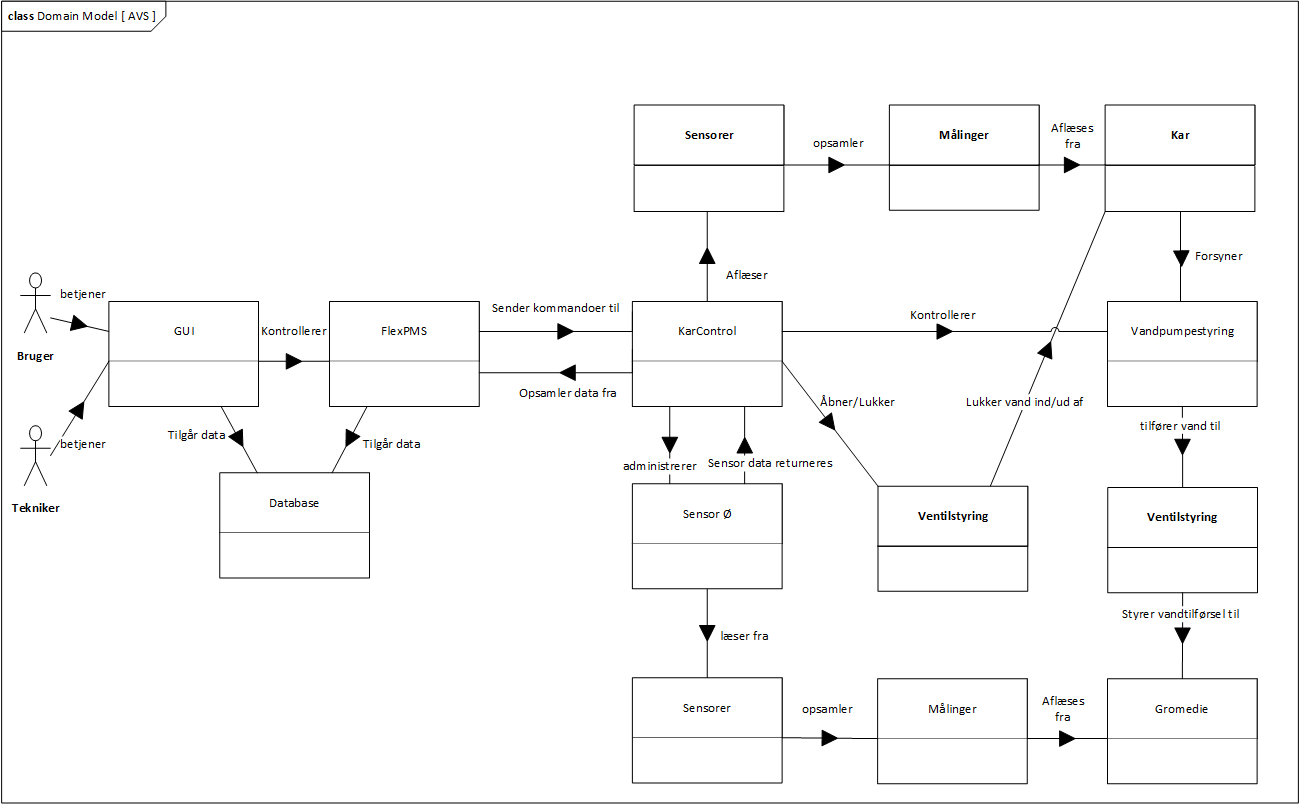
\includegraphics[width=0.82\textwidth]{Systemarkitektur/System/AVS_domain_model.png}
	\label{fig:System BDD}
	\caption{Domain model af AVS}
\end{figure}



\subsection{System BDD}

\begin{figure}[H]
	\centering
	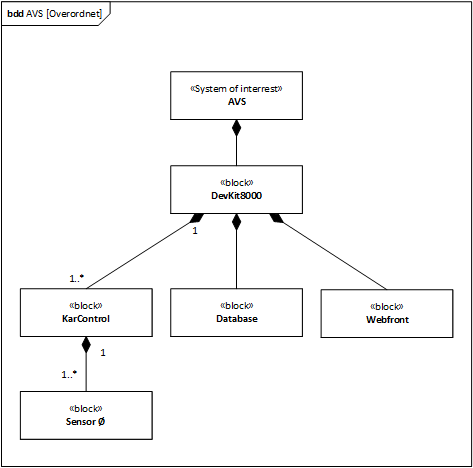
\includegraphics[width=0.82\textwidth]{Systemarkitektur/System/AVS_SystemdiagramBDD.png}
	\label{fig:System BDD}
	\caption{Block Definition Diagram af AVS}
\end{figure}



\subsection{Allokeringsdiagram}

\begin{figure}[H]
	\centering
	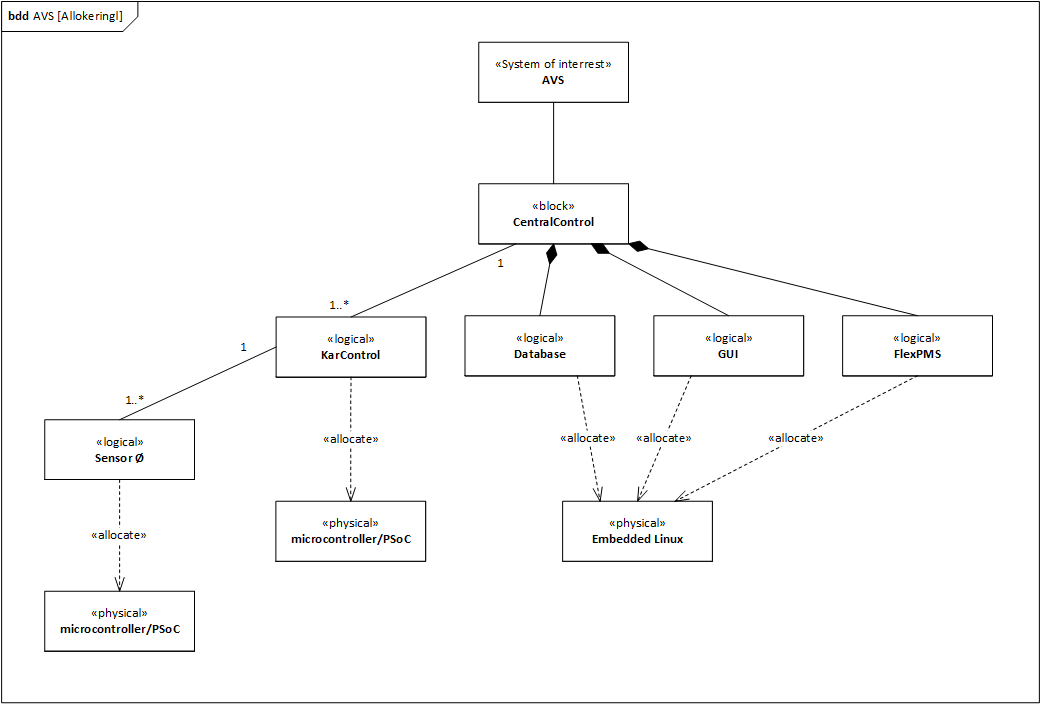
\includegraphics[width=0.82\textwidth]{Systemarkitektur/System/AVS_Allokeringsdiagram.png}
	\label{fig:System BDD}
	\caption{Allokeringsdiagram af AVS}
\end{figure}









\newpage

\section{Kar Control diagrammer}

%!TEX root = ../../main.tex

\subsection{KarControl BDD}
\systemBDD{0.82}{KarControl}

\subsubsection{KarGruppe}
KarGruppe er den overordnede betegnelse for et vandkar med tilførende pH-værdi og gødningskoncentration. KarGruppen består af diverse sensorer og aktuatorer, og styrer et vilkårligt antal Sensor Ø’er. KarGruppen er styret af en controller, KarControl.

\subsubsection{Indløbsventil}
Indløbsventilen åbner og lukker for vandtilføjelsen til karret. Den bruges i forbindelse med, at der skal fyldes vand på karret. Det antages, at indløbsventilen er tilsluttet en vandforsyning, som altid er åben.

\subsubsection{Afløbsventil}
Afløbsventilen åbner og lukker for, at vand kan løbe ud af karret. Den bruges i forbindelse med, at karret skal tømmes.

\subsubsection{pH-Sensor}
pH-sensoren målet pH-værdien af gødningsblandingen i karret.

\subsubsection{Vandpumpe}
Vandpumpen pumper vand fra karret ud til Sensor Ø’erne.

\subsubsection{Flowmåler}
Flowmåleren måler mængden af vand, som tilføres karret gennem Indløbsventilen.

\subsubsection{PSU}
PSU (Power Supply Unit) forsyner de andre blokke med 12V og 5V.

\subsection{KarControl IBD}
\systemIBD{0.82}{KarControl}{KarControl}

\subsubsection{RSIn}
RSConverter konverterer mellem RS485 og UART 232 når der skal kommunikeres med CentralControl.

\subsubsection{RSOut}
RSConverter konverterer mellem RS485 og UART 232 når der skal kommunikeres med Sensor Ø'er.

\subsection{KarControlForsyning IBD}
Der er lavet et separat forsynings IBD som viser forbindelserne fra blokken PSU til resten af blokkene og omverdenen.
\begin{figure}[H]
	\centering
	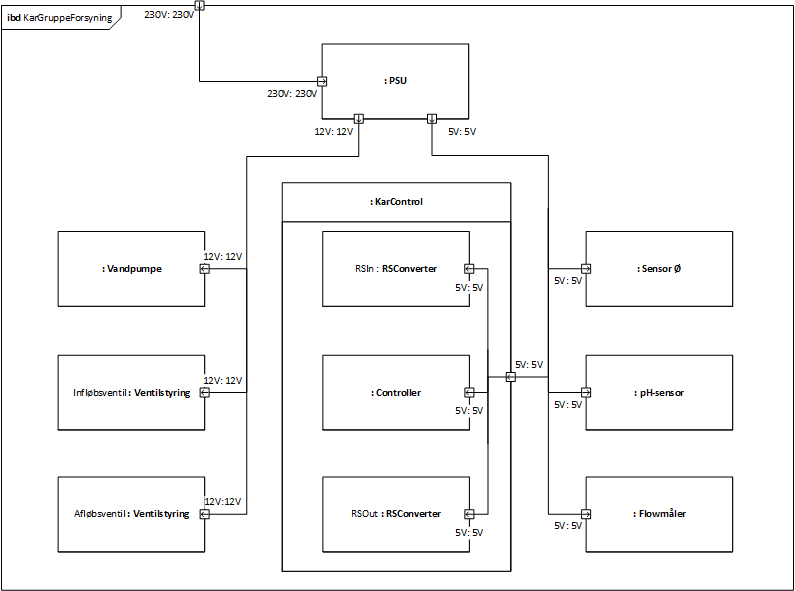
\includegraphics[scale=0.7]{Systemarkitektur/KarControl/KarControlForsyning_IBD.png}
	\label{fig:KarControlForsyning}
	\caption{IBD over forsyningsforbindelser til KarControl}
\end{figure}

%\subsection{KarControl Allokeringsdiagram}
%\systemAllokeringsDiagram{0.82}{KarControl}{KarControl}

\subsection{Signalbeskrivelser KarControl}
\systemSignaler{KarControl} {
KarBus				& RS485 bus til kommunikation mellem enheder &	 	& Differentielt bussystem  \\
OeBus				& RS485 bus til kommunikation mellem enheder &	 	& Differentielt bussystem  \\
Data485				& RS485 bus til kommunikation mellem enheder &	 	& internt signal   \\
Data232				& RS485 konverteret til logisk niveau		 &	 	& Signal efter konvertering  \\
EnableIndløb		& Signal til at lukke vand ind i kar		 & 0-5V	& Signal til at styre magnetventil   \\
EnableAfløb			& Signal til at lukke vand ud af kar		 & 0-5V	& Signal til at styre magnetventil	\\
EnableVandpumpe		& Signal til styring af vandpumpe			   	     & 0-5V & PWM styret signal	\\
Puls				& Takttæller af flow				   	 	 & 0-5V & 	\\
pH					& Analog signal fra pH måler			 	 & fra -420 til 420 mV  & Analogt signal	\\
Indløb				& vandstyring i kar							 &    	& Til at lukke vand ind i kar	\\
Afløb				& vandstyring i kar	 						 &   	& Til at lukke vand ud af kar	\\
Dossering			& vandstyring til planter					 &      & Til at dosere vand til planterne	\\
230V				& El-nettet som forsyner PSU				 & 230V	& \\
12V					& Forsyning til pumper og ventiler			 & 12V	& \\
5V					& Forsyning til systemets logiske kredsløb	 & 5V	& \\
}

\newpage

\section{SensorØ diagrammer}

%%!TEX root = ../../main.tex

\subsection{Sensoroe BDD}

\begin{figure}[H]
	\centering
	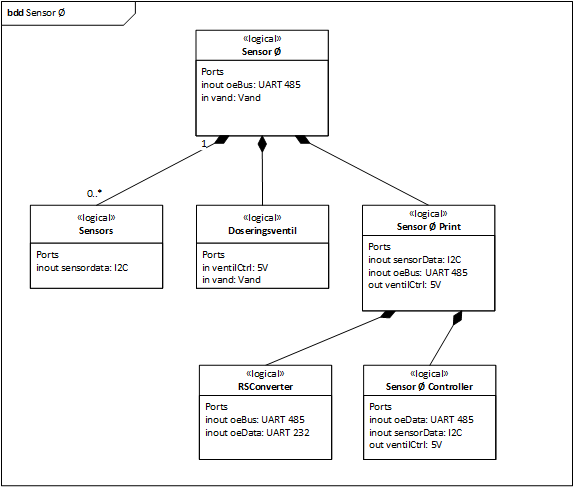
\includegraphics[width=0.82\textwidth]{Systemarkitektur/Sensoroe/Sensoroe_BDD.png}
	\label{fig:Sensoroe BDD}
	\caption{Block Definition Diagram af Sensoroe}
\end{figure}

\subsubsection*{Sensor Ø Control}
Sensor Ø Control tager imod kommandoer fra KarControl, som instruerer omkring åbning og lukning af Doseringsventil. KarControl anmoder også om, at Sensor Ø Control skal sende måledata fra sensors, som er tilkoblet Sensor Ø’en.

\subsubsection{Doseringsventil}
Doseringsventilen åbner og lukker for vandtilførslen til planterne i området omkring Sensor Ø’en, som Doseringsventilen er tilkoblet. Når KarControl tænder for Vandpumpen kan de enkelte Sensor Ø’ers Doseringsventiler være åbne eller lukkede alt efter, om planterne omkring Sensor Ø’en har brug for vand.

\subsubsection{Sensor}
Sensor er en generalisering af alle slags sensorer, som kan tilsluttes Sensor Ø’en. Vilkårligt mange sensorer kan tilkobles en bus, og kommunikere med Sensor Ø Control gennem en standardiseret protokol. Sensor kan kun aflevere målinger når de bliver bedt om at levere dem.

\subsection{Sensoroe IBD}

\begin{figure}[H]
	\centering
	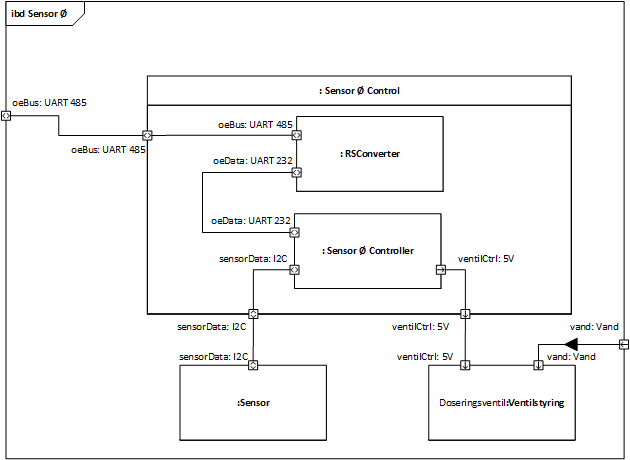
\includegraphics[width=0.82\textwidth]{Systemarkitektur/Sensoroe/Sensoroe_IBD.png}
	\label{fig:Sensoroe BDD}
	\caption{Internal Block Diagram af Sensoroe}
\end{figure}



\subsection{Sensoroe Allokeringsdiagram}

\begin{figure}[H]
	\centering
	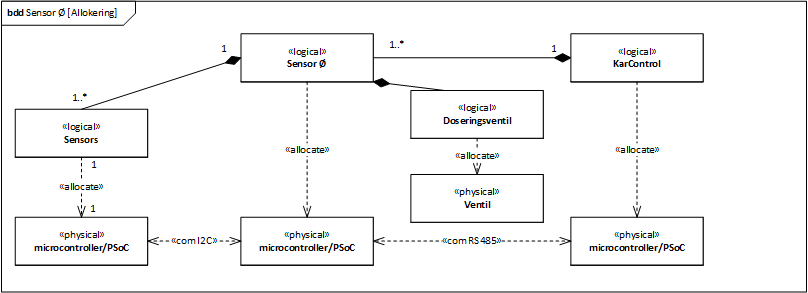
\includegraphics[width=0.82\textwidth]{Systemarkitektur/Sensoroe/Sensoroe_Allokeringsdiagram.png}
	\label{fig:Sensoroe BDD}
	\caption{Allokeringsdiagram af Sensoroe}
\end{figure}

\newpage

\section{pH-sensor diagrammer}

%%!TEX root = ../../main.tex

Til pH måling har vi bygget vores egen sensor ved hjælp af en pH-probe.

\subsection{pH-sensor BDD}

I forhold til signaler er proben ret nem at have med at gøre da den selv producere en spænding i forhold til den væske der måles på pH værdi.

\begin{figure}[H]
	\centering
	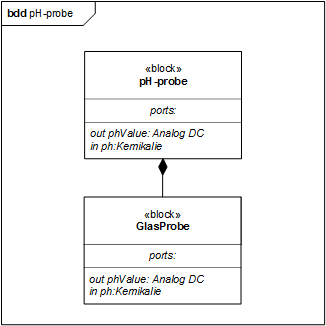
\includegraphics[width=0.7\textwidth]{Systemarkitektur/Sensor_pH/pH_Probe_BDD.png}
	\label{fig:pH-sensor BDD}
	\caption{Block Definition Diagram af pH-sensor}
\end{figure}



\subsection{pH-sensor IBD}

Igen ses simpliciteten da pH proben bare interagere med kemikalium og herefter producere en spænding.

\begin{figure}[H]
	\centering
	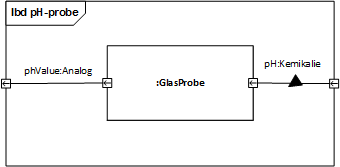
\includegraphics[width=0.7\textwidth]{Systemarkitektur/Sensor_pH/pH_Probe_IBD.png}
	\label{fig:pH-sensor IBD}
	\caption{Internal Block Diagram af pH-sensor}
\end{figure}




\newpage

\section{jordfugtigheds-sensor diagrammer}

%!TEX root = ../../main.tex

Jordfugtigheds sensoren måler en strøm igennem jorden. Denne strøm vil variere med hensyn til fugtigheden som derfor vil resultere i en spændingsændring på indgangen af analog til digital converteren. Denne spænding bruges til at udregne fugtigheden i procent

\subsection{pH-sensor BDD}

\begin{figure}[H]
	\centering
	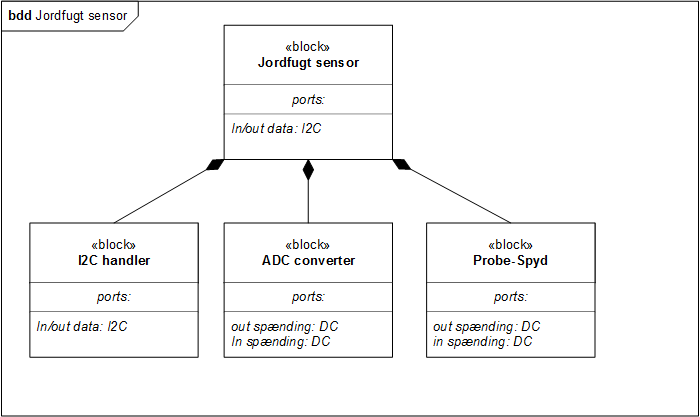
\includegraphics[width=0.82\textwidth]{Systemarkitektur/Sensor_jordfugtighed/JordFugt_probe_BDD.png}
	\label{fig:pH-sensor BDD}
	\caption{Block Definition Diagram af pH-sensor}
\end{figure}



\subsection{pH-sensor IBD}

\begin{figure}[H]
	\centering
	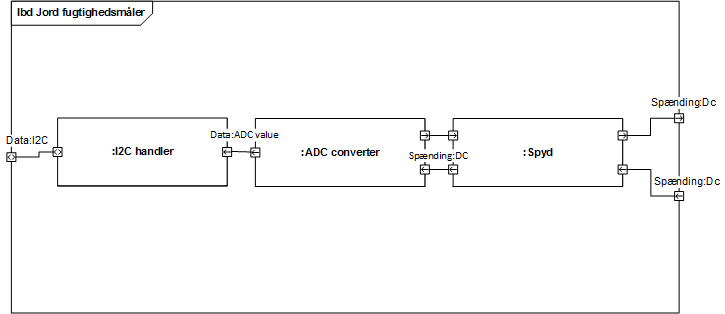
\includegraphics[width=0.82\textwidth]{Systemarkitektur/Sensor_jordfugtighed/JordFugt_probe_IBD.png}
	\label{fig:pH-sensor IBD}
	\caption{Internal Block Diagram af pH-sensor}
\end{figure}

\newpage

\section{Ventil diagrammer}

%!TEX root = ../../main.tex

\subsection{Ventilstyring BDD}

\begin{figure}[H]
	\centering
	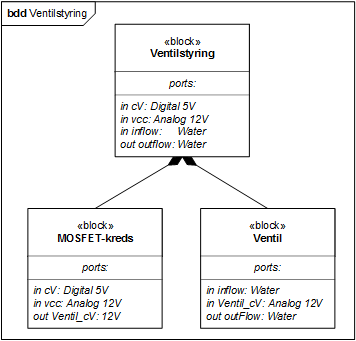
\includegraphics[width=0.82\textwidth]{Systemarkitektur/Ventiler/Ventilstyring_BDD.png}
	\label{fig:Ventilstyring BDD}
	\caption{Block Definition Diagram af Ventilstyring}
\end{figure}



\subsection{System IBD}

\begin{figure}[H]
	\centering
	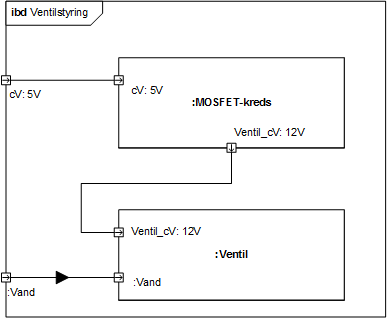
\includegraphics[width=0.82\textwidth]{Systemarkitektur/Ventiler/Ventilstyring_IBD.png}
	\label{fig:Ventilstyring IBD}
	\caption{Internal Block Diagram af Ventilstyring}
\end{figure}



\subsection{System Flowchart}

\begin{figure}[H]
	\centering
	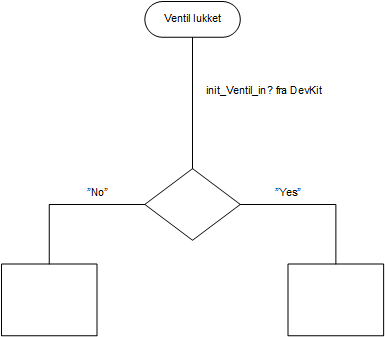
\includegraphics[width=0.82\textwidth]{Systemarkitektur/Ventiler/Ventilstyring_Flowchart.png}
	\label{fig:Ventilstyring FC}
	\caption{Flowchart af Ventilstyring}
\end{figure}

\newpage

\section{RS485 Converter diagrammer}

\newpage

\section{Teknologi undersøgelser}

%!TEX root = ../../main.tex
%!TEX root = ../../../main.tex


Det der RS485 er bare lovely


%!TEX root = ../../../main.tex
\subsection{Ventiler}
Følgende krav er opstillet for indløb- og afløbsventil, samt doseringsventilerne 

\begin{table}[h]
	\begin{tabular}{ l l l }
		1. 	& Tolerance for Vandtryk:   	& Skal kunne klare min. 2 bar \\
		2. 	& Forsyningsspænding: 			& Skal kunne benytte 12V DC \\
		3.	& Tolerance for Temp: 			& Skal kunne operere ved 45 C \\
		4.	& Flow-regulering: 				& Skal kunne levere min. 0.5 liter/min
	\end{tabular}
\end{table}

Det vigtigste krav til indløb- og afløb- og doseringsventilerne er, at de bør være rated til at kunne klare de tryk, der påhviler dem. 
For indløbsventilen gælder følgende grænseflader: 

\begin{table}[h]
	\begin{tabular}{ l l l }
		1. 	& Vandtilførsel udefra   		& \\
		2. 	& Vandkaret: 					&
	\end{tabular}
\end{table}

Her bør opmærksomheden primært henledes på vandtrykket udefra. 
Der tages udgangspunkt i den alm. Vandhane, her i er vandtrykket som standard på omkring 2 bar . 
Derfor skal den ventil der vælges som min. kunne klare et tryk 2 bar. 
For afløbsventilen gælder følgende grænseflade: 

\begin{table}[h]
	\begin{tabular}{ l l l }
		1. 	& Vandkaret:  					& \\
		2. 	& Afløb: 						&
	\end{tabular}
\end{table}

Her bør opmærksomheden henledes på trykket i vandkaret, som her maksimalt kan være på 1 bar, afløbet bidrager ikke med noget tryk og kan ignoreres. 

For doseringsventilen gælder følgende grænseflade
For afløbsventilen gælder følgende grænseflade: 

\begin{table}[h]
	\begin{tabular}{ l l l }
		1. 	& Vandtryk i doseringsslange:  			& \\
		2. 	& Udløb: 						&
	\end{tabular}
\end{table}

Her bør opmærksomheden henledes på trykket i doseringsslangen, dette skabes af doseringspumpen og kan max være på 2 bar, udløbet bidrager ikke med noget tryk og kan ignoreres. 


Der blev undersøgt flere typer ventiler i forhold til de ovenstående krav, og det blev besluttet at benytte en magnet-ventil til opgaven. Dette blev primært besluttet på baggrund af styringsmetoden af en magnetventil, denne passer til designet at systemet.  
Den valgte model blev: 
Hydraelectric Magnetventil, 2 Porte, NC, 12 V dc, 1/2tommer.
Datablad for den findes under Datablade. 


%!TEX root = ../../../main.tex
\subsection{Doseringspumpe}
Følgende krav er opstillet for doseringspumpen.  

\begin{table}[h]
	\begin{tabular}{ l l l }
		1. 	& Tolerance for Vandtryk:   	& Skal kunne klare min. 2 bar \\
		2. 	& Forsyningsspænding: 			& Skal kunne benytte 12V DC \\
		3.	& Tolerance for Temp: 			& Skal kunne operere ved 45 C \\
		4.	& Flow-regulering: 				& Skal kunne levere min. 0.5 liter/min
	\end{tabular}
\end{table}

Her bør opmærksomheden primært henledes på vandtrykket der kan opstå i slangen, imellem doseringspumpen og doseringsventilerne, hvis ingen af disse ikke er åbne når pumpen tændes.
Dette problem vil praktisk blive løst software-wise, således at det ikke er muligt at tænde for pumpen med mindre at min. Én af de tilkoblede ventiler er åbne.  

Der blev undersøgt flere typer pumper i forhold til de ovenstående krav, og det blev besluttet at benytte en inline pumpe til opgaven. Dette blev primært besluttet på baggrund af dens performance og forsyning, denne passer til designet at systemet.  
Den valgte model blev: 
Biltema inline Pump, 17l/min, DC12V, 3A, 
Datablad for den findes under Datablade. 
 

%!TEX root = ../../../main.tex
\subsection{Flowsensor}
Følgende krav er opstillet for flowsensoren 

\begin{table}[h]
	\begin{tabular}{ l l l }
		1. 	& Tolerance for Vandtryk:   	& Skal kunne klare min. 2 bar \\
		2. 	& Forsyningsspænding: 			& Skal kunne benytte 12V DC \\
	\end{tabular}
\end{table}

Det vigtigste krav til flowsensoren er, at den bør være rated til at kunne klare det tryk, der påhviler den. 
For flowsensoren gælder følgende grænseflader: 

\begin{table}[h]
	\begin{tabular}{ l l l }
		1. 	& Vandtilførsel udefra   		& \\
		2. 	& Vandkaret: 					&
	\end{tabular}
\end{table}

Her bør opmærksomheden primært henledes på vandtrykket udefra. 
Der tages udgangspunkt i den alm. Vandhane, her i er vandtrykket som standard på omkring 2 bar . 
Derfor skal den ventil der vælges som min. kunne klare et tryk 2 bar. 
For afløbsventilen gælder følgende grænseflade: 

\begin{table}[h]
	\begin{tabular}{ l l l }
		1. 	& Vandkaret:  					& \\
		2. 	& Afløb: 						&
	\end{tabular}
\end{table}

Her bør opmærksomheden primært henledes på vandtrykket udefra. 
Der tages udgangspunkt i den alm. Vandhane, her i er vandtrykket som standard på omkring 2 bar . 
Derfor skal den flowsensor der vælges som min. kunne klare et tryk 2 bar. 

Der blev undersøgt flere typer ventiler i forhold til de ovenstående krav, og det blev besluttet at benytte en YF-S201 Hall Effekt flow sesnor. Dette blev primært besluttet på baggrund af måden hvorpå den afgiver sine målinger, dette passer til designet at resten systemet.  
Den valgte model blev: 
Sea, 2 Porte, YF-S201 Hall Effekt flowsensor, 12v DC,  1/2tommer.
Datablad for den findes under Datablade. 

\fixme{der skal indsættes resten af teknologi undersøgelserne}

